
\newcommand{\nomedoc}{Specifica Tecnica}
\newcommand{\versione}{0.4}
\newcommand{\versioneglossario}{1.0}
\newcommand{\versionenormeprogetto}{1.0}
\newcommand{\nomefile}{SpecificaTecnica-\versione.pdf}
\newcommand{\datacreazione}{2 Dicembre 2010}
\newcommand{\datamodifica}{28 Gennaio 2011}
\newcommand{\stato}{formale}
\newcommand{\uso}{interno}
\newcommand{\redazione}{Mandolo Andrea}
\newcommand{\verifica}{---}
\newcommand{\approvazione}{---}
\newcommand{\distribuzione}{
VT.G \\
& Prof. Vardanega Tullio\\
& Prof. Cardin Riccardo }

% FUNZIONI TIPOGRAFICHE
\newcommand{\co}{\texttt} % courier
\newcommand{\bo}{\textbf} % bold
\newcommand{\pr}{\par\medskip} % paragrafo spaziato
\newcommand{\sca}{\textsc} % small caps

\documentclass[a4paper,12pt]{report}
% 10pt,11pt,12pt
% titlepage, notitlepage -> per dare inizio o no ad una nuova pagina dopo titolo
% twoside -> per dire se fronte-retro
\usepackage[latin1]{inputenc}
% per caratteri accentati
\usepackage[italian]{babel}
% per regole sintattiche italiane
\usepackage[bookmarks=true, pdfborder={0 0 0 0}]{hyperref}
% per collegamenti ipertestuali
\usepackage{graphicx}
% per inserimento immagini

% \usepackage{enumerate}
% per personalizzare elenchi puntati

\usepackage[hmargin=2cm]{geometry} %margine 2 cm
%\geometry{options varie}

% comandi per gestire meglio header e footer
\usepackage{fancyhdr}  % header e footer
\usepackage{totpages}
\pagestyle{fancy}
\renewcommand{\headrulewidth}{0.4pt}
\renewcommand{\footrulewidth}{0.4pt}

\setlength{\headheight}{1.2cm} % NON TOCCARE
\setlength{\voffset}{-1.5cm} % NON TOCCARE
\setlength{\textheight}{666pt} % NON TOCCARE
\setlength{\footskip}{60pt}
\setlength{\parindent}{0pt} % INDENTAZIONE

\lhead{\nomedoc\  (ver. \versione)}
\chead{}
\rhead{
\includegraphics[height=1cm]{img/netmus.png}}
\lfoot{
\includegraphics[height=0.8cm]{img/logo.png}}
\cfoot{}
\rfoot{\thepage}

\usepackage{titlesec}
\titleformat{\chapter}{\normalfont\huge\bfseries}
{\thechapter}{20pt}{\Huge}

\usepackage{rotating}   % PER TABELLE E AMBIENTI RUOTATI
\usepackage{array}
\usepackage{color}
\usepackage{colortbl}  % VARIE PER GESTIRE I COLORI
\definecolor{Orange}{RGB}{255,127,0}   % ARANCIO ACCES0
\definecolor{orange}{RGB}{255,207,80}  % ARANCIO TENUE

\addtocontents{toc}{\protect\thispagestyle{fancy}}  % PER INDICI CON + PAGINE
\usepackage[font=it]{caption}    % PER RENDERE CORSIVE LE DIDASCALIE
\usepackage{eurosym}  % PER SIMBOLO EURO

% \usepackage{listings}   per codice sorgente

\author{VT.G - Valter Texas Group}

\begin{document}

\pagenumbering{Roman} % INIZIO NUMERAZIONE ARABA

\vspace*{1cm}
\begin{center}

\begin{LARGE} \sca{Federico Baron} \end{LARGE}\\
\vspace{0.5cm}
\begin{Large}
\emph{fede.baron.89@gmail.com} \end{Large}\\
\vspace*{1cm} 
\includegraphics[width=5cm]{img/logo.png}\\
\vspace{0.5cm}
\begin{Large} \emph{``Comunicazione Aumentata/Alternativa per Giovani Ospiti
della Terapia Intensiva Pediatrica''} \end{Large}\\
\vspace{3cm}
\begin{Large} \sca{\nomedoc} \end{Large}\\
\end{center}
\vspace{1cm}

% INFORMAZIONI DOCUMENTO
\begin{center}
\begin{tabular}{r|l}
\hline & \\
\bo{Nome} & \nomefile \\
\bo{Versione attuale} & \versione \\
\bo{Data creazione} & \datacreazione \\
\bo{Data ultima modifica} & \datamodifica \\
\bo{Redazione} & \redazione \\
& \\\hline
\end{tabular}
\end{center}
\newpage

% REGISTRO MODIFICHE
\section*{Registro delle modifiche}

\begin{longtable}{|p{0.13\textwidth}|c|p{0.2\textwidth}|p{0.46\textwidth}|}
\hline
\rowcolor{orange} \bo{Data} & \bo{Versione} & \bo{Autore} & \bo{Descrizione} \\
\hline
\endhead
\hline
\endfoot

28/01/2011 & 0.4 & Mandolo Andrea & Inserita traccia dell'intero capitolo 2.\\
\hline
27/01/2011 & 0.3 & Baron Federico & Redazione del capitolo 2.2.1 Deisgn
patterns.\\
\hline
27/01/2011 & 0.2 & Mandolo Andrea & Inserita presentazione dell'architettura
generale del sistema.\\
\hline
21/01/2011 & 0.1 & Mandolo Andrea & Creato documento iniziale.\\

\end{longtable}

% INDICE
\tableofcontents

\chapter*{Sommario}
Il presente documento fornisce la descrizione ad alto livello dell'architettura
del sistema Netmus, riservando particolare attenzione alle motivazioni e ai
metodi utilizzati per l'identificazione delle principali componenti, alla loro
struttura, funzione e alle relazioni d'uso. Vengono infine presentati una stima
della fattibilit\`a e delle risorse necessarie e il tracciamento delle
componenti sui requisiti, descritti in dettaglio nel documento
\emph{AnalisiDeiRequisiti}.


\thispagestyle{fancy} % serve perche' nelle pagine di inizio Chapter esca header e footer
\pagenumbering{arabic} % INIZIO NUMERAZIONE NORMALE
\rfoot{\thepage\ di \pageref{TotPages}}
\addcontentsline{toc}{chapter}{Sommario}

\chapter{Introduzione}
\thispagestyle{fancy} % serve perche' nelle pagine di inizio Chapter esca header e footer

\section{Scopo del documento}
Lo scopo della Specifica Tecnica \`e quello di illustrare le scelte progettuali
che il gruppo ha deciso di seguire nella realizzazione del prodotto. Viene
presentata, pur restando ad alto livello, la gerarchia dei package, delle loro
connessioni e delle principali classi di cui essi si compongono.


\section{Scopo del prodotto}
Il progetto \underline{NetMus} nasce con lo scopo di realizzare un sistema
software basato su \underline{cloud} \underline{computing}, per memorizzare
informazioni di brani musicali in profili utente online.\\ Tali informazioni vengono estratte da
dispositivi musicali o di archiviazione \underline{USB} al momento della loro connessione.

\section{Glossario}
Il Glossario \`e definito con un documento a parte
(\emph{Glossario-\versioneglossario.pdf}). Tutti i termini caratterizzati da
\underline{questa sottolineatura} sono ivi definiti.\\
Verr\`a sottolineata solamente la prima occorrenza di ciascun
termine presente nel Glossario, per non compromettere la leggibilit\`a del documento.

\section{Riferimenti}

\subsection{Normativi} % oppure rif. a Norme di progetto con leggi e tutto
\begin{itemize}
  \item ISO/IEC 12207:1995 - Cicli di vita software
  \item ISO/IEC 9126:2001 - Quality Model
  \item \emph{NormeDiProgetto-\versionenormeprogetto.pdf} che regola e
  accompagna tutti i documenti ufficiali.
\end{itemize}
\newpage
\subsection{Informativi}
\begin{itemize}
  \item Capitolato d'appalto CO2-NETMUS del corso di Ingegneria del Software
  A.A. 2010/11 :\\
  \url{http://www.math.unipd.it/~tullio/IS-1/2010/Progetto/NetMus.pdf}
  \item Slide delle lezioni del corso:\\
  \url{http://www.math.unipd.it/~tullio/IS-1/2010/}
  \item Verbale intervista proponente:\\
  \co{allegato Verbale-1.0.pdf}
  \item Sistema di cloud Google App Engine:\\
  \url{http://code.google.com/intl/it/appengine/}
\end{itemize}


\chapter{Definizione del Prodotto}
\section{Metodo e formalismo di specifica}
I diagrammi delle classi illustrati in questo capitolo (utilizzando il
linguaggio di modellazione e specifica UML) definiscono la struttura ad alto
livello del sistema Netmus a partire da una visione macroscopica del sistema,
scendendo via via nel dettaglio.

\section{Presentazione dell'architettura generale del sistema.}

\subsection{Design patterns utilizzati}
Nei seguenti paragrafi sono presentati i design patterns utilizzati per
sviluppare l'architettura di NetMus. Alcuni di questi derivano dall'utilizzo
delle tecnologie GAE e GWT che forniscono dei frameworks che implementano
patterns considerati best practices per queste particolari tecnologie.

\subsubsection{L'importanza dei design patterns in NetMus}
La via intrapresa da VT.G nello sviluppo del sistema NetMus comprende il forte
utilizzo dei design patterns al fine di produrre un software al pi\`u
possibile manutenibile ed estendibile e che quindi mantenga un ciclo di
vita equilibrato. 
I design patterns inibiscono l'ispirazione dei programmatori dove
questa non \`e necessaria e piuttosto forniscono un modo universalmente
riconosciuto di produrre software ben architettato e facilmente manutenibile.
MVP in particolare \`e il pattern pi\`u utilizzato sulla piattaforma Google Web
Toolkit ed \`e quindi sostenuto egregiamente da alcuni strumenti offerti da
Google.

\newpage
\subsubsection{Model View Presentation (MVP) }
La potenza di questo pattern architetturale \`e quella di separare tre
importantissime componenti riducendo l'accoppiamento e facilitando i processi di
verifica e validazione:
\begin{itemize}
  \item{\bo{View} }
  costituisce l'interfaccia utente che comprende tutte le componenti utili alla
  visualizzazione.
  \item{\bo{Model} }
  contiene i dati che dovranno essere mostrati. 
  \item{\bo{Presenter} }
  \`e la componente fondamentale, si occupa di mandare i dati del model
  all'interfaccia e viceversa. Pu\`o inoltre gestire gli eventi scatenati da
  altre parti del sistema o avviare i propri grazie alla comunicazione diretta
  con un event bus.

\end{itemize}    
\begin{figure}[!h]
\centering
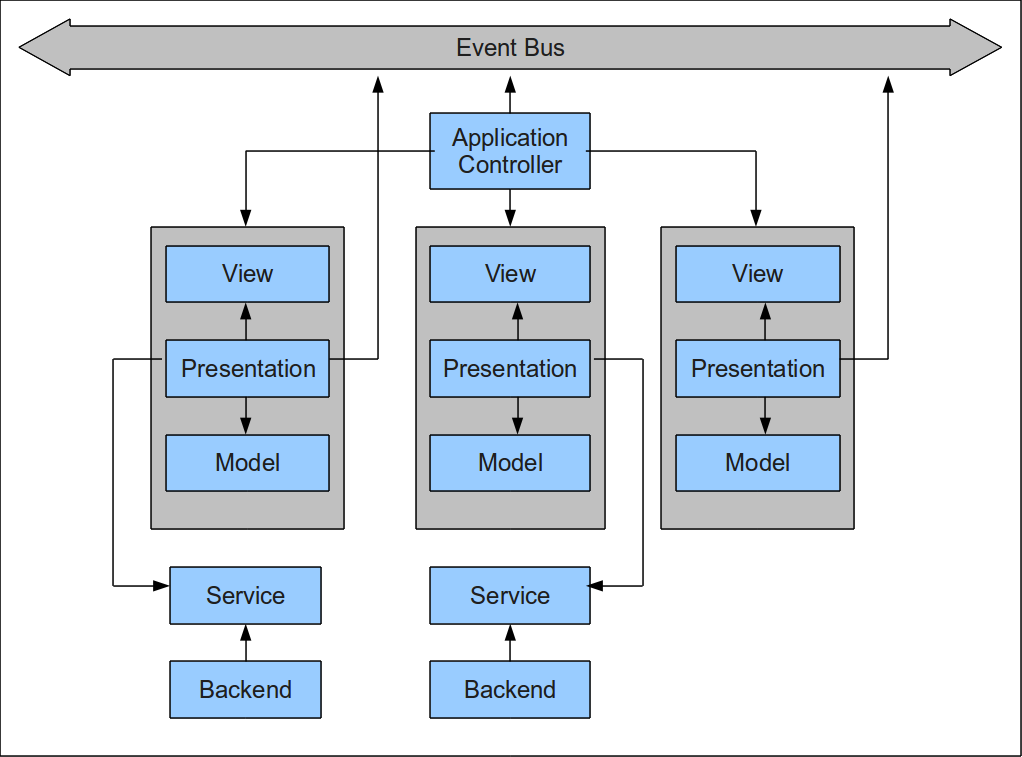
\includegraphics[width=8.5cm]{img/ST/mvp.png}
\caption{Architettura tipica di MVP utilizzando Google Web Toolkit}
\end{figure}

Nel nostro caso questo design pattern sar\`a implementato con il framework MVP con
Activities e Places offerto da GWT 2.1 che semplifica la gestione di alcuni
aspetti consolidati di MVP. In questo framework le Activities svolgono il ruolo
di Presenter e i Places rappresentano gli stati della UI.
\begin{itemize}
  \item{\bo{Activity} }
  \`e l'analogo di presenter in MVP tradizionale. Non contiene alcun componente
  grafico ed il suo avvio e la sua terminazione sono gestite da un
  ActivityManager.
  \item{\bo{Place} }
  un Place in GWT 2.1 rappresenta un particolare stato della UI e viene
  utilizzato anche per tenere una history degli URL che \`e fondamentale per una
  Web Application.

\end{itemize} 
\begin{figure}[h]
\centering
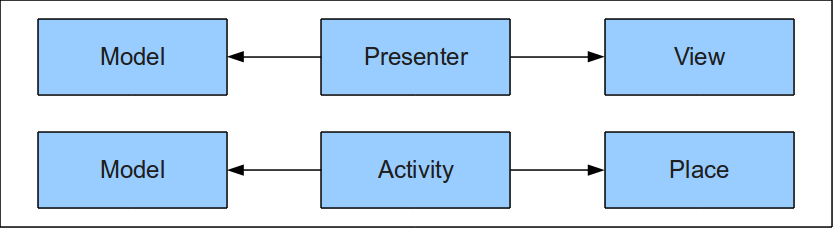
\includegraphics[width=7cm]{img/ST/mvpap.png}
\caption{Comparazione tra MVP tradizionale e MVP con Activities e Places}
\end{figure}

\newpage

\subsubsection{Data Access Object (DAO)  e  Data Transfer Object (DTO)}
\begin{figure}[h]
\centering
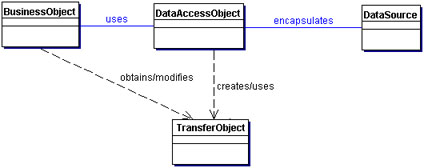
\includegraphics[width=9cm]{img/ST/daodto.png}
\caption{Diagramma UML delle classi che descrive la struttura dell'utilizzo
simultaneo dei patterns DAO e DTO}
\end{figure}
Questi patterns vengono introdotti all'interno della componente model di MVP e
riguardano gli oggetti utilizzati per l'incapsulamento dei dati nelle
comunicazioni tra client, server e database. 
Il DAO (Data Access Object) \`e un pattern semplice ma fondamentale per
stratificare ed isolare gli accessi al database dalla parte logica
dell'applicazione, nel nostro caso le Activity di MVP. L'implementazione \`e
fondamentalmente una classe che rappresenta un'entit\`a tabellare di un database.
Questi oggetti estratti dal database in alcuni casi possono essere utilizzati
per la comunicazione con i clients ma hanno pesanti restrizioni dovute alla
grande quantit\`a di informazioni e procedure che contengono, per questo motivo
abbiamo deciso di affiancare a DAO anche il pattern Data Transfer Object. Gli
oggetti DTO saranno quelli che verranno scambiati nella comunicazione tra client
e server con il vantaggio di essere pi\`u essenziali dei DAO e la possibilit\`a di
costituire dei pacchetti su misura per la comunicazione. La logica del
tracciamento tra DAO e DTO sar\`a a carico degli oggetti DAO.
\\
Per questo scopo GWT2.1 propone un potente framework per gestire la
comunicazione tra client e server, Request Factory, che implementa i patterns
precedentemente descritti. Abbiamo deciso per\`o di non utilizzarlo, progettando
una nostra implementazione, a causa della documentazione insufficente fornita
da Google.

\newpage
\subsubsection{Abstract factory}
Un abstract factory \`e rappresentata da un'interfaccia che permette di creare dei
prodotti senza specificare classi concrete.

\begin{figure}[h]
\centering
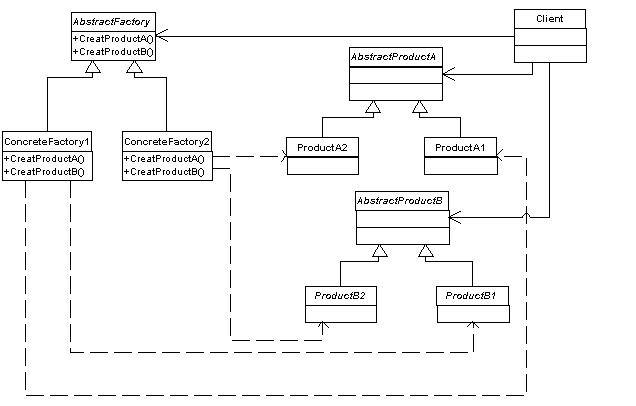
\includegraphics[width=13cm]{img/ST/as.png}
\caption{Diagramma UML delle classi che descrive la struttura tradizionale di
Abstract factory}
\end{figure}
Nello specifico lo utilizzeremo per rendere facilmente configurabile il nostro
sistema. L'interfaccia ClientFactory sar\`a utilizzata per ottenere le
intefacce degli elementi architetturali necessari alla nostra applicazione come
ad esempio l'event bus e le varie UI.
Per caricare le differenti implementazioni di ClientFactory a seconda delle
peculiarit\`a dell'utente che vi accede \`e molto conveniente utilizzare il GWT
deferred binding offerto dal toolkit stesso.
Il pattern in questione verr\`a utilizzato per una evidente convenienza in termini
di estendibilit\`a per il futuro anche se allo stadio attuale la factory
implementata sar\`a solamente una.

\newpage
\subsubsection{Data Access Object (DAO)  e  Data Transfer Object (DTO)}
\begin{figure}[h]
\centering
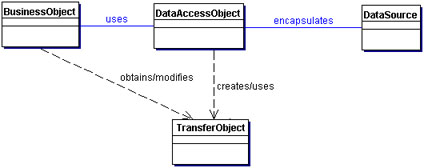
\includegraphics[width=9cm]{img/ST/daodto.png}
\caption{Diagramma UML delle classi che descrive la struttura dell'utilizzo
simultaneo dei patterns DAO e DTO}
\end{figure}
Questi patterns vengono introdotti all'interno della componente model di MVP e
riguardano gli oggetti utilizzati per l'incapsulamento dei dati nelle
comunicazioni tra client, server e database. 
Il DAO (Data Access Object) \`e un pattern semplice ma fondamentale per
stratificare ed isolare gli accessi al database dalla parte logica
dell'applicazione, nel nostro caso le Activity di MVP. L'implementazione \`e
fondamentalmente una classe che rappresenta un'entit\`a tabellare di un database.
Questi oggetti estratti dal database in alcuni casi possono essere utilizzati
per la comunicazione con i clients ma hanno pesanti restrizioni dovute alla
grande quantit\`a di informazioni e procedure che contengono, per questo motivo
abbiamo deciso di affiancare a DAO anche il pattern Data Transfer Object. Gli
oggetti DTO saranno quelli che verranno usati nella comunicazione tra client
e server con il vantaggio di essere pi\`u essenziali dei DAO, sono pacchetti su
misura per la comunicazione. La logica del tracciamento tra DAO e DTO sar\`a a
carico degli oggetti DAO.

\newpage
\subsubsection{Singleton}
\begin{figure}[h]
\centering
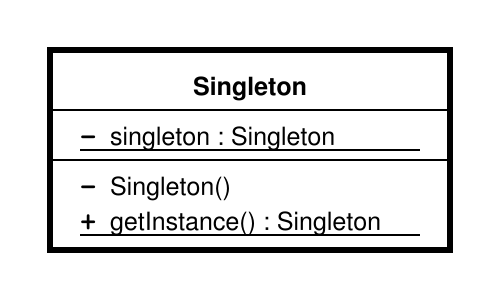
\includegraphics[width=8cm]{img/ST/Singleton.png}
\caption{Diagramma UML delle classi che descrive l'implementazione del design
pattern Singleton}
\end{figure}
Singleton \`e un design pattern creazionale che ha lo scopo di assicurare
l'esistenza di una sola istanza di una certa classe ed avere un punto di accesso
globale a quest'ultima. 
L'implementazione di Singleton diminuisce in generale l'accoppiamento del
sistema.
Utilizzeremo questo pattern per una classe (Persistent manager factory) che si
occupera di creare degli speciali oggetti introdotti da JDO per la
comunicazione con il database (query). \`E molto importante che venga instanziata una sola
istanza di Persistent manager factory e che questa sia visibile all'intero
dell'intero lato server del sistema NetMus. 

\newpage
\subsection{Diagrammi UML dei Package}
Il sistema Netmus sar\`a principalmente formato dai seguenti package:
\begin{figure}[h]
  \centering
  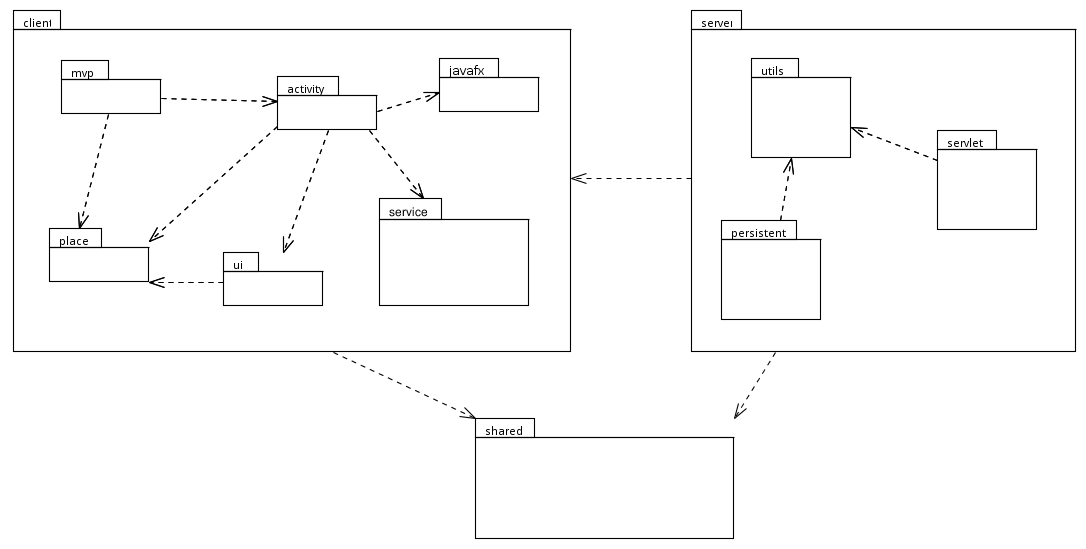
\includegraphics[width=16cm]{img/ST/PackageGeneric.png}
\caption{Diagramma dei package principali di Netmus.}
\end{figure}

\begin{itemize}
  \item Package \emph{client} : definisce la parte client del programma
  \begin {itemize}
    \item Package \emph{client.ui} : comprende l'insieme di viste del sistema,
    rispettando il framework \emph{MVP with Place and Activity}. Ci sar\`a una
    interfaccia per ogni vista, per dare la possibilit\`a di creare in futuro
    pi\`u implementazioni differenti a seconda del dispositivo client;
    \item Package \emph{client.activity} : rappresenta l'insieme di classi
    controllori che formano la logica del sistema. Esse mandano dati aggiornati alle
    viste, gestiscono le richieste delle viste e possono inoltre gestire
    richieste provenienti da altre componenti e mandare eventi propri nell'event-bus;
    \item Package \emph{client.place} : comprende l'insieme di classi Place i
    quali rappresentano un URL associato ad una vista. Gestiscono i parametri
    agganciati all'URL con un Tokenizer interno;
    \item Package \emph{client.mvp} : comprende un ActivityMapper e
    un PlaceHistoryManager che mappano per ogni Place la sua corrispondente
    Activity e gestiscono la cronologia dei Place;
    \item Package \emph{client.service} : rappresenta l'insieme di interfaccie
    che offrono un servizio di comunicazione col server tramite \underline{GWT
    RPC};
    %----------------- TOGLIERE FORSE --------------------
    \item Package \emph{client.javafx} : contiene l'interfacciamento alla
    applet JavaFX di estrazione dei TAG dagli Mp3 da dispositivi multimediali del client;
    %-------------------------------------------------------
  \end {itemize}
  \item Package \emph{server} : rappresenta la parte server di Netmus
  \begin{itemize}
    \item Package \emph{server.persistent} : comprende tutte le classi che
    rappresentano un entit\`a JDO (Java Data Object), le quali usate per lo scambio dati tra
    server e Google Datastore;
    \item Package \emph{server.servlet} : comprende tutte le servlet utilizzate
    per interfacciarsi a servizi esterni (es. Google Authentication, YouTube);
    \item Package \emph{server.utils} : comprende classi di utilit\`a per
    svolgere attivit\`a interne al server di varie tipologie;
  \end{itemize}
  \item Package \emph{shared} :  contiene classi condivise tra client e server,
  che verrano anch'esse compilate in JavaScript da GWT, come tutto il package
  client. La maggior parte saranno gli oggetti di trasferimento che
  aderiscono al pattern DTO.
\end{itemize}

\chapter{Descrizione dei singoli componenti}
\section{Package client}
\begin{figure}[h]
  \centering
  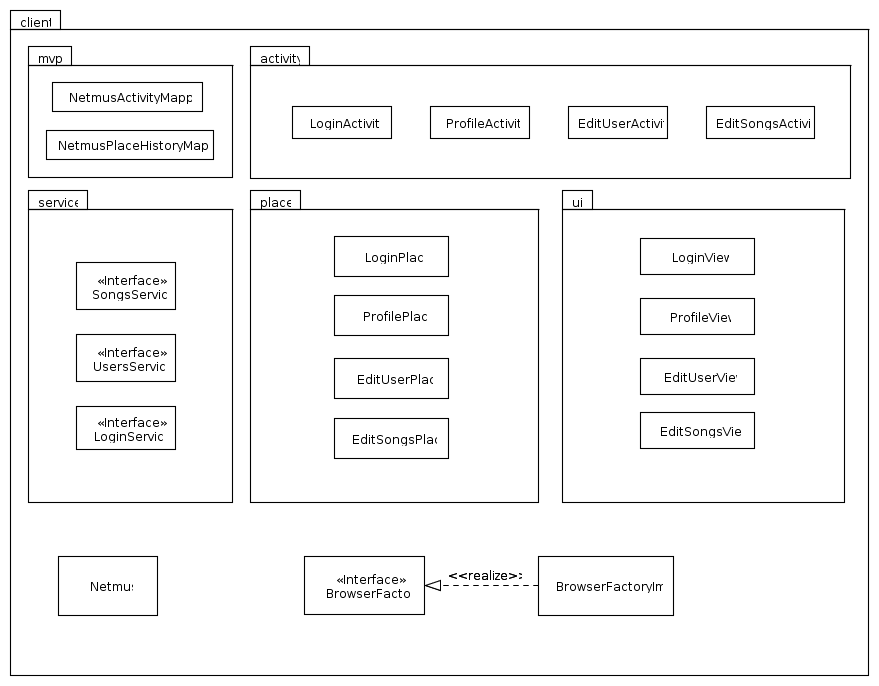
\includegraphics[width=16cm]{img/ST/ClassClient.png}
\caption{Diagramma delle classi del package client.}
\end{figure}

\newpage
\subsection*{Tipo, obiettivo e funzione del componente} % LASCIARE WARNING
Il package client rappresenta la parte del sistema con la quale l'utente pu\`o
interagire. Tutte le sue classi ed i suoi sottopackage saranno compilati in
JavaScript da GWT, prima che il sistema venga depositato nel dominio
\emph{appspot.com} di Google. Contiene la classe \underline{Entry Point}
\co{Netmus}.

\subsection*{Relazioni d'uso di altre componenti}
Il package client utilizza i DTO nel package shared.

\subsection*{Interfacce con altre componenti}
Nessuna.

\subsection*{Attivit\`a svolte e dati trattati}
Le attivit\`a svolte dalle sue classi verranno qui di seguito descritte.

\subsection{Classe Netmus}
\subsubsection*{Tipo, obiettivo e funzione del componente}
\subsubsection*{Relazioni d'uso di altre componenti}
\subsubsection*{Interfacce con altre componenti}
\subsubsection*{Attivit\`a svolte e dati trattati}

\subsection{Classe ClientFactoryImpl (\emph{Abstract Factory})}
\subsubsection*{Tipo, obiettivo e funzione del componente}
In Netmus \`e disponibile un'unica implementazione dell'intefaccia
ClientFactory, poich\`e per il momento non \`e contemplato un utilizzo di
alternative all'interfaccia utente desktop.
Nella classe si definiscono le propriet\`a di un vista (desktop) del
sistema.

\subsubsection*{Relazioni d'uso di altre componenti}
La classe utilizza \co{EventBus}, \co{PlaceController}, \co{LoginView},
\co{ProfileView}, \co{EditUserView} e
\co{EditSongView}.
\subsubsection*{Interfacce con altre componenti}
\co{Netmus} crea l'istanza della classe. L'interfaccia \co{ClientFactory} \`e
utilizzata da \co{ActivityMapper} e successivamente dalle \co{Activity} per
l'utilizzo dell'EventBus.
\subsubsection*{Attivit\`a svolte e dati trattati}
La classe si occupa di istanziare l'event bus, il place controller e le varie
view. L'event bus gestisce le comunicazioni tra componenti, il place
controller permette la navigazione tra i Place ed \`e si occupa di avvisare
l'utente prima del passaggio ad uno stato differente.


\newpage
\section{Package client.ui} % LASCIARE WARNING
\subsection*{Tipo, obiettivo e funzione del componente}
\subsection*{Relazioni d'uso di altre componenti}
\subsection*{Interfacce con altre componenti}
\subsection*{Attivit\`a svolte e dati trattati}

\subsection{Classe LoginView}
\subsubsection*{Tipo, obiettivo e funzione del componente}
Il sistema mette a disposizione una vista per l'autenticazione e la
registrazione degli utenti Netmus.
\subsubsection*{Relazioni d'uso di altre componenti}
La classe istanzia oggetti di tipo \co{Place} che definiscono gli stati attuali
della vista.
\subsubsection*{Interfacce con altre componenti}
La vista viene creata da \co{ClientFactory} e \`e settata ed utilizzata dalle
varie \co{Activity}.
\subsubsection*{Attivit\`a svolte e dati trattati}
Mette a disposizione gli strumenti per l'immissione dei dati utente e per le
comunicazioni operative.

\subsection{Classe ProfileView}
\subsubsection*{Tipo, obiettivo e funzione del componente}
\subsubsection*{Relazioni d'uso di altre componenti}
\subsubsection*{Interfacce con altre componenti}
\subsubsection*{Attivit\`a svolte e dati trattati}

\subsection{Classe EditUserView}
\subsubsection*{Tipo, obiettivo e funzione del componente}
\subsubsection*{Relazioni d'uso di altre componenti}
\subsubsection*{Interfacce con altre componenti}
\subsubsection*{Attivit\`a svolte e dati trattati}

\subsection{Classe EditSongsView}
\subsubsection*{Tipo, obiettivo e funzione del componente}
\subsubsection*{Relazioni d'uso di altre componenti}
\subsubsection*{Interfacce con altre componenti}
\subsubsection*{Attivit\`a svolte e dati trattati}

\newpage
\section{Package client.activity} % LASCIARE WARNING
\subsection*{Tipo, obiettivo e funzione del componente}
\subsection*{Relazioni d'uso di altre componenti}
\subsection*{Interfacce con altre componenti}
\subsection*{Attivit\`a svolte e dati trattati}

\subsection{Classe LoginActivity}
\subsubsection*{Tipo, obiettivo e funzione del componente}
\subsubsection*{Relazioni d'uso di altre componenti}
\subsubsection*{Interfacce con altre componenti}
\subsubsection*{Attivit\`a svolte e dati trattati}

\subsection{Classe ProfileActivity}
\subsubsection*{Tipo, obiettivo e funzione del componente}
\subsubsection*{Relazioni d'uso di altre componenti}
\subsubsection*{Interfacce con altre componenti}
\subsubsection*{Attivit\`a svolte e dati trattati}

\subsection{Classe EditUserActivity}
\subsubsection*{Tipo, obiettivo e funzione del componente}
\subsubsection*{Relazioni d'uso di altre componenti}
\subsubsection*{Interfacce con altre componenti}
\subsubsection*{Attivit\`a svolte e dati trattati}

\subsection{Classe EditSongsActivity}
\subsubsection*{Tipo, obiettivo e funzione del componente}
\subsubsection*{Relazioni d'uso di altre componenti}
\subsubsection*{Interfacce con altre componenti}
\subsubsection*{Attivit\`a svolte e dati trattati}

\newpage
\section{Package client.place} % LASCIARE WARNING
\subsection*{Tipo, obiettivo e funzione del componente}
\subsection*{Relazioni d'uso di altre componenti}
\subsection*{Interfacce con altre componenti}
\subsection*{Attivit\`a svolte e dati trattati}

\subsection{Classe LoginPlace}
\subsubsection*{Tipo, obiettivo e funzione del componente}
\subsubsection*{Relazioni d'uso di altre componenti}
\subsubsection*{Interfacce con altre componenti}
\subsubsection*{Attivit\`a svolte e dati trattati}

\subsection{Classe ProfilePlace}
\subsubsection*{Tipo, obiettivo e funzione del componente}
\subsubsection*{Relazioni d'uso di altre componenti}
\subsubsection*{Interfacce con altre componenti}
\subsubsection*{Attivit\`a svolte e dati trattati}

\subsection{Classe EditUserPlace}
\subsubsection*{Tipo, obiettivo e funzione del componente}
\subsubsection*{Relazioni d'uso di altre componenti}
\subsubsection*{Interfacce con altre componenti}
\subsubsection*{Attivit\`a svolte e dati trattati}

\subsection{Classe EditSongsPlace}
\subsubsection*{Tipo, obiettivo e funzione del componente}
\subsubsection*{Relazioni d'uso di altre componenti}
\subsubsection*{Interfacce con altre componenti}
\subsubsection*{Attivit\`a svolte e dati trattati}

\newpage
\section{Package client.mvp} % LASCIARE WARNING
\subsection*{Tipo, obiettivo e funzione del componente}
\subsection*{Relazioni d'uso di altre componenti}
\subsection*{Interfacce con altre componenti}
\subsection*{Attivit\`a svolte e dati trattati}

\subsection{Classe NetmusActivityMapper}
\subsubsection*{Tipo, obiettivo e funzione del componente}
\subsubsection*{Relazioni d'uso di altre componenti}
\subsubsection*{Interfacce con altre componenti}
\subsubsection*{Attivit\`a svolte e dati trattati}

\subsection{Classe NetmusPlaceHistoryMapper}
\subsubsection*{Tipo, obiettivo e funzione del componente}
\subsubsection*{Relazioni d'uso di altre componenti}
\subsubsection*{Interfacce con altre componenti}
\subsubsection*{Attivit\`a svolte e dati trattati}

\newpage
\section{Package client.service} % LASCIARE WARNING
\subsection*{Tipo, obiettivo e funzione del componente}
\subsection*{Relazioni d'uso di altre componenti}
\subsection*{Interfacce con altre componenti}
\subsection*{Attivit\`a svolte e dati trattati}

\subsection{Classe SongsService}
\subsubsection*{Tipo, obiettivo e funzione del componente}
\subsubsection*{Relazioni d'uso di altre componenti}
\subsubsection*{Interfacce con altre componenti}
\subsubsection*{Attivit\`a svolte e dati trattati}

\subsection{Classe UsersService}
\subsubsection*{Tipo, obiettivo e funzione del componente}
\subsubsection*{Relazioni d'uso di altre componenti}
\subsubsection*{Interfacce con altre componenti}
\subsubsection*{Attivit\`a svolte e dati trattati}

\subsection{Classe LoginService}
\subsubsection*{Tipo, obiettivo e funzione del componente}
\subsubsection*{Relazioni d'uso di altre componenti}
\subsubsection*{Interfacce con altre componenti}
\subsubsection*{Attivit\`a svolte e dati trattati}

%--------------- FORSE -------------------------------
\section{Package client.javafx} % LASCIARE WARNING
\subsection*{Tipo, obiettivo e funzione del componente}
\subsection*{Relazioni d'uso di altre componenti}
\subsection*{Interfacce con altre componenti}
\subsection*{Attivit\`a svolte e dati trattati}
%------------------------------------------------------
\newpage
\section{Package server} % LASCIARE WARNING
\subsection*{Tipo, obiettivo e funzione del componente}
\subsection*{Relazioni d'uso di altre componenti}
\subsection*{Interfacce con altre componenti}
\subsection*{Attivit\`a svolte e dati trattati}

\subsection{Classe SongsServiceImpl}
\subsubsection*{Tipo, obiettivo e funzione del componente}
\subsubsection*{Relazioni d'uso di altre componenti}
\subsubsection*{Interfacce con altre componenti}
\subsubsection*{Attivit\`a svolte e dati trattati}

\subsection{Classe UsersServiceImpl}
\subsubsection*{Tipo, obiettivo e funzione del componente}
\subsubsection*{Relazioni d'uso di altre componenti}
\subsubsection*{Interfacce con altre componenti}
\subsubsection*{Attivit\`a svolte e dati trattati}

\subsection{Classe LoginServiceImpl}
\subsubsection*{Tipo, obiettivo e funzione del componente}
\subsubsection*{Relazioni d'uso di altre componenti}
\subsubsection*{Interfacce con altre componenti}
\subsubsection*{Attivit\`a svolte e dati trattati}

\subsection{Classe LoginHelper}
\subsubsection*{Tipo, obiettivo e funzione del componente}
\subsubsection*{Relazioni d'uso di altre componenti}
\subsubsection*{Interfacce con altre componenti}
\subsubsection*{Attivit\`a svolte e dati trattati}

\newpage
\subsection{Classe PMF (Singleton)}
\subsubsection*{Tipo, obiettivo e funzione del componente}
\subsubsection*{Relazioni d'uso di altre componenti}
\subsubsection*{Interfacce con altre componenti}
\subsubsection*{Attivit\`a svolte e dati trattati}

\section{Package server.peristent} % LASCIARE WARNING
\subsection*{Tipo, obiettivo e funzione del componente}
\subsection*{Relazioni d'uso di altre componenti}
\subsection*{Interfacce con altre componenti}
\subsection*{Attivit\`a svolte e dati trattati}

\subsection{Classe User (da decidere nomi e tipi di DAO)}
\subsubsection*{Tipo, obiettivo e funzione del componente}
\subsubsection*{Relazioni d'uso di altre componenti}
\subsubsection*{Interfacce con altre componenti}
\subsubsection*{Attivit\`a svolte e dati trattati}

\subsection{Classe . . . . (da decidere nomi e tipi di DAO)}
\subsubsection*{Tipo, obiettivo e funzione del componente}
\subsubsection*{Relazioni d'uso di altre componenti}
\subsubsection*{Interfacce con altre componenti}
\subsubsection*{Attivit\`a svolte e dati trattati}

\newpage
\section{Package server.servlet} % LASCIARE WARNING
\subsection*{Tipo, obiettivo e funzione del componente}
\subsection*{Relazioni d'uso di altre componenti}
\subsection*{Interfacce con altre componenti}
\subsection*{Attivit\`a svolte e dati trattati}

\subsection{Classe LoginSuperServlet}
\subsubsection*{Tipo, obiettivo e funzione del componente}
\subsubsection*{Relazioni d'uso di altre componenti}
\subsubsection*{Interfacce con altre componenti}
\subsubsection*{Attivit\`a svolte e dati trattati}

\subsection{Classe LoginGoogleServlet}
\subsubsection*{Tipo, obiettivo e funzione del componente}
\subsubsection*{Relazioni d'uso di altre componenti}
\subsubsection*{Interfacce con altre componenti}
\subsubsection*{Attivit\`a svolte e dati trattati}

\subsection{Classe LoginGoogleCallbackServlet}
\subsubsection*{Tipo, obiettivo e funzione del componente}
\subsubsection*{Relazioni d'uso di altre componenti}
\subsubsection*{Interfacce con altre componenti}
\subsubsection*{Attivit\`a svolte e dati trattati}

\subsection{Classe YouTubeServlet (da decidere tipo di servlet)}
\subsubsection*{Tipo, obiettivo e funzione del componente}
\subsubsection*{Relazioni d'uso di altre componenti}
\subsubsection*{Interfacce con altre componenti}
\subsubsection*{Attivit\`a svolte e dati trattati}

\newpage
\subsection{Classe TaggingServlet(da decidere . . .)}
\subsubsection*{Tipo, obiettivo e funzione del componente}
\subsubsection*{Relazioni d'uso di altre componenti}
\subsubsection*{Interfacce con altre componenti}
\subsubsection*{Attivit\`a svolte e dati trattati}

\section{Package server.utils} % LASCIARE WARNING
\subsection*{Tipo, obiettivo e funzione del componente}
\subsection*{Relazioni d'uso di altre componenti}
\subsection*{Interfacce con altre componenti}
\subsection*{Attivit\`a svolte e dati trattati}

\subsection{Classe AuthenticationProvider}
\subsubsection*{Tipo, obiettivo e funzione del componente}
\subsubsection*{Relazioni d'uso di altre componenti}
\subsubsection*{Interfacce con altre componenti}
\subsubsection*{Attivit\`a svolte e dati trattati}

\subsection{Classe ServletUtils}
\subsubsection*{Tipo, obiettivo e funzione del componente}
\subsubsection*{Relazioni d'uso di altre componenti}
\subsubsection*{Interfacce con altre componenti}
\subsubsection*{Attivit\`a svolte e dati trattati}

\subsection{Classe Utils}
\subsubsection*{Tipo, obiettivo e funzione del componente}
\subsubsection*{Relazioni d'uso di altre componenti}
\subsubsection*{Interfacce con altre componenti}
\subsubsection*{Attivit\`a svolte e dati trattati}

\newpage
\section{Package shared} % LASCIARE WARNING
\subsection*{Tipo, obiettivo e funzione del componente}
\subsection*{Relazioni d'uso di altre componenti}
\subsection*{Interfacce con altre componenti}
\subsection*{Attivit\`a svolte e dati trattati}

\subsection{Classe 'Tipo'DTO  (decidere tipi DTO ecc)}
\subsubsection*{Tipo, obiettivo e funzione del componente}
\subsubsection*{Relazioni d'uso di altre componenti}
\subsubsection*{Interfacce con altre componenti}
\subsubsection*{Attivit\`a svolte e dati trattati}

\subsection{Classe . . . .  (decidere tipi DTO ecc)}
\subsubsection*{Tipo, obiettivo e funzione del componente}
\subsubsection*{Relazioni d'uso di altre componenti}
\subsubsection*{Interfacce con altre componenti}
\subsubsection*{Attivit\`a svolte e dati trattati}

\chapter{Stime di fattibilit\`a e di bisogno di risorse}

\chapter{Tracciamento della relazione componenti - requisiti}

\listoftables
\addcontentsline{toc}{chapter}{Indice Tabelle}
\listoffigures
\addcontentsline{toc}{chapter}{Indice Figure}
\end{document}
